\section{Dispositivo di RTINGS}
Il sito di recensioni RTINGS\footnote{\href{https://rtings.com/}{https://rtings.com/}} ha sviluppato un proprio dispositivo per eseguire diversi tipi di misurazioni sui display: tempi di latenza, tempi di risposta dei pixel, errore di transizione causato dall'overdrive, e altro.

Purtroppo non sono note informazioni sul dispositivo stesso, ma è visibile in alcune fotografie presenti nelle recensioni, come quella in figura \ref{fig:rtings_device}. Sembra essere un sistema composto da un'MCU e da un sensore di luminosità. Non è noto come i dati raccolti dal sensore vengano analizzati (manualmente o da un programma apposito).

\begin{figure}[h]
	\centering
	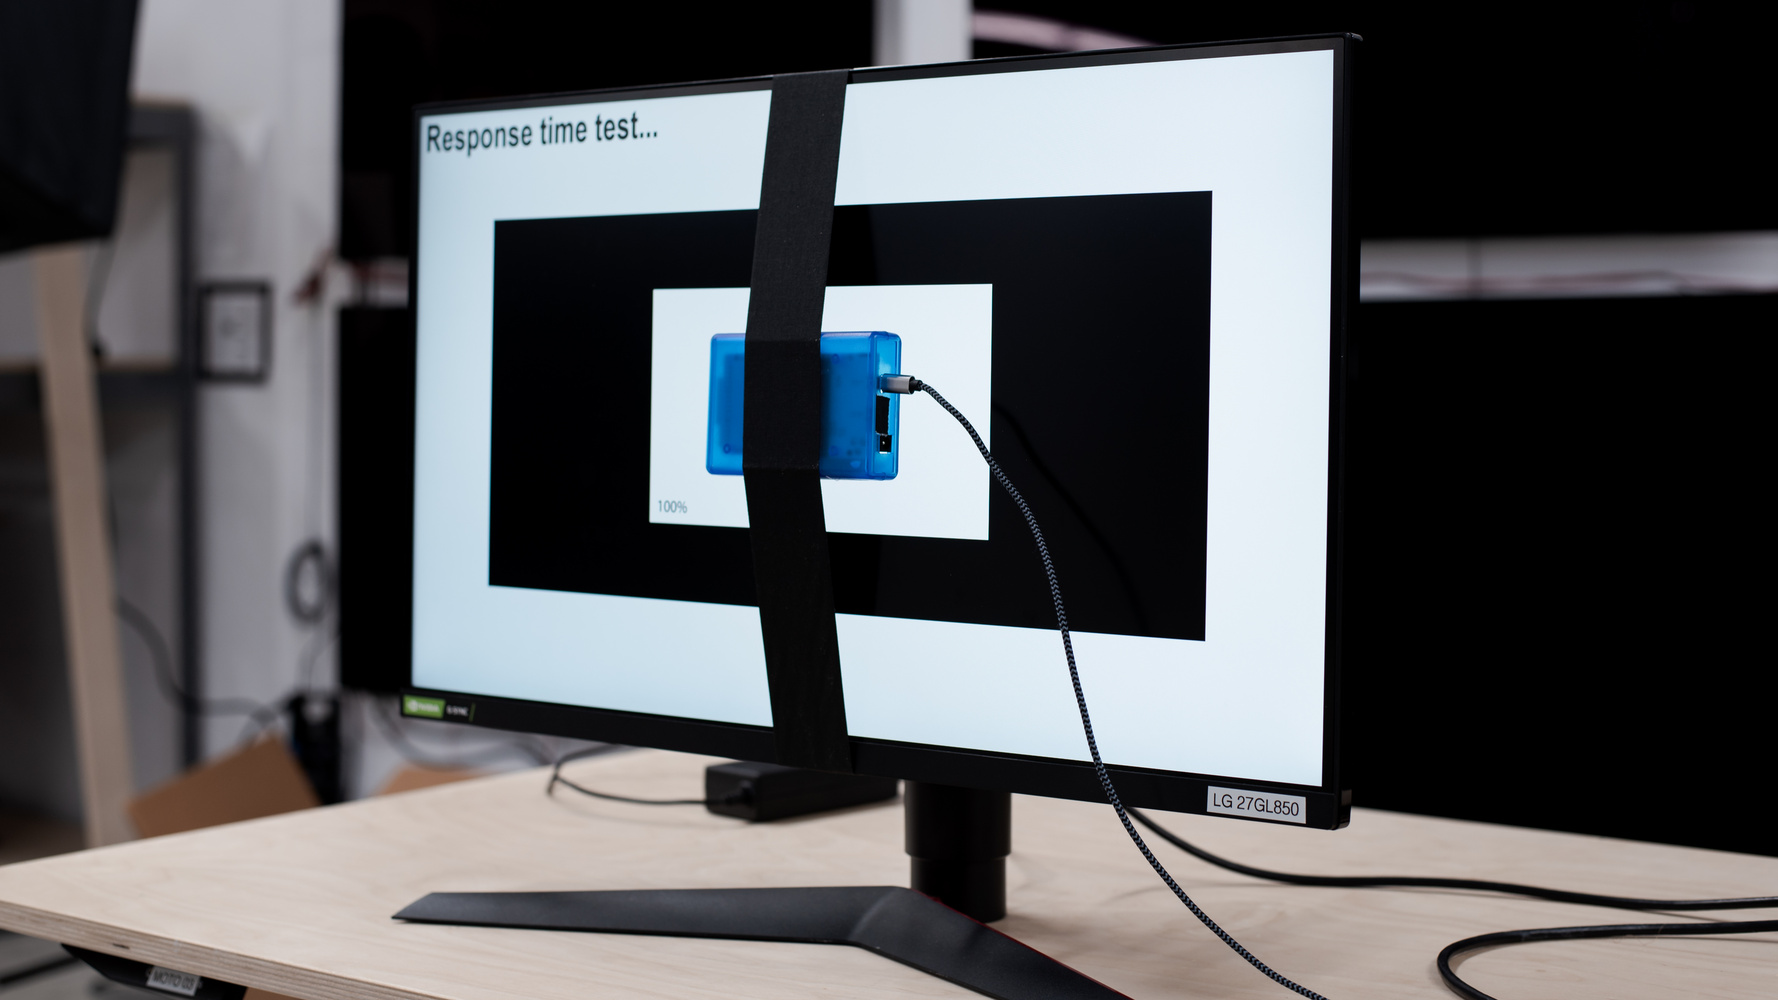
\includegraphics[width=\textwidth]{Chapter02/res/rtings_device.jpg}
	\caption{Il dispositivo di RTINGS}
	\label{fig:rtings_device}
\end{figure}

Altri test nelle recensioni presenti sul sito vengono invece svolti utilizzando un colorimetro e DisplayCAL: luminosità, contrasto, curve di gamma, gamut, temperatura del bianco, e altro.

Alcuni test infine sono eseguiti manualmente con una telecamera, come quello sugli angoli di visione.

Questo conclude il capitolo sullo stato dell'arte. I capitoli successivi si concentrano sul progetto OpenLDAT.
